\section{Zielsetzung}
Im Versuch wird das Relaxationsverhalten beim Entaldevorgang eines Kondensators
in einem RC-Tiefpass auf sein Frequenzverhalten (bei niedrigen und hohen Frequenzen),
sowie die Phasenverschiebung zwischen Kondensator und Generatorspannung hin untersucht.
Weiter wird der Tiefpass auf seine Eigenschaft als Integrator betrachtet.

\section{Theorie}
Das Relaxationsverhalten eines Systems ist dadurch gekennzeichnet, dass es, nachdem
es von seinem Ausgangszustand entfernt wurde, nicht oszillatorisch in diesen wieder
zurückkehrt.
Im Versuch wird als Beispiel für das Relaxationsverhalten der Auf- und Entladevorgang
eines Kondensators in einem RC-Tiefpass betrachtet.

\begin{figure}[h!]
  \centering
  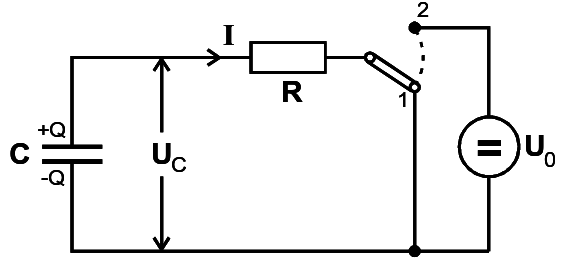
\includegraphics[scale=0.7]{kondensator.png}
  \caption{RC-Kreis \cite{Quelle}}
\end{figure}
Für den Aufladevorgang eines Kondensators ergibt sich mit den Anfangsbedingungen
\begin{align*}
  Q(0) = 0  &&&& Q(\infty) = C U_0
\end{align*}
folgende Gleichung für $Q(t)$
\begin{equation*}
  Q(t) = C U_0 (1 - exp(\frac{-t}{RC}))
\end{equation*}
Dabei bezeichnet C die Kapazität des Kondensators, R den Widerstand und $Q_0$ die
Ladung des Kondesators zum Zeitpunkt $t = 0$.
Die Gleichung
\begin{equation*}
  Q(t) = Q_0(1-exp(\frac{-t}{RC}))
\end{equation*}
beschreibt den Entladevorgang des Kondensators. Das Produkt aus $R$ und $C$ wird
dabei als Zeitkonstante bezeichnet und beschreibt, wie schnell das System in seinen
Endzustand $G(\inf)$ relaxiert.
Werden die Geschehnisse am RC Kreis mit einem von außen sinusförmig angeregten System
in der Mechanik verglichen, so lassen sich einige Analogien finden. Zum einen weisen
die Schwingungsgleichungen Parallelen auf, zum anderen ist das Verhalten bei einem
Widerstand sehr ähnlich.
Wird nun ein RC-Kreis mit der Wechselspannung
\begin{equation*}
  U(t) = U_0 cos(\omega t)
\end{equation*}
angeregt, kann eine Phasenverschiebung zwischen der Eingangsspannung und der
Spannung am Kondensator bei zunehmender Frequenz beobachtet werden.
Betrachtet man jedoch sehr hinreichend geringe Frequenzen für $\omega$, also
$\omega << \frac{1}{RC}$, so wird sich beobachten lassen, dass die Spannung am
Kondensator $U_\symup{C}(t)$ ungefähr gleich der Eingangsspannung $U(t)$ sin wird.
Durch Erhöhen der Eingangsfrequenz wird eine Phasenverschiebung zwischen den beiden
Spannungen erzwungen. Hierbei hinkt der Auf- und Entladevorgang am Kondensator
zeitlich hinter der Erregerspannung zurück.
Als Formel für die Phasenverschiebung $\phi$ in Abhängigkeit der Frequenz $\omega$
ergibt sich:
\begin{equation*}
  \phi(\omega) = arctan(-\omega RC)
\end{equation*}.
Für niedrige Frequenzen nähert sich die Phasenverschiebung, wie bereits erwähnt,
dem Wert 0. Für hohe Frequenzen wird sich die Phasenverschiebung asymptotisch dem
Wert $\frac{\pi}{2}$ nähern.
Des weiteren können mit Hilfe der Gleichung
\begin{equation*}
  A (\omega) = \frac{U_0}{\sqrt{1 + \omega^2 R^2 C^2}}
\end{equation*}
Aussagen über die Änderung der Amplitude mit zunehmender Erregerfrequenz getroffen
werden. Geht $\omega$ gegen 0, so gilt $A(\omega) \to U_0$, geht $\omega$ gegen $\inf$,
gilt dann umgekehrt: $A(\omega) \to 0$.
Das Verhalten von Tiefpässen ist dadurch charakterisiert, dass Frequenzen, für die gilt
$\omega >> \frac{1}{RC}$, immer weiter gesperrt werden, wohingegen niedrigere Frequenzen
$\omega << \frac{1}{RC}$ durchgelassen werden.
Außer der Eigenschaft als Tiefpass, kann ein RC-Schaltkreis auch als Integrator der
Eingangsspannung dienen, solange die Erregerfrequenz ausreichend groß ist:
$\omega >> \frac{1}{RC}$.
Dabei wird gelten:
\begin{equation*}
  U_\symup{C}(t) = \frac{1}{RC}\int_0^t U(t') dt'
\end{equation*}.
\newpage
\section{Durchführung}
Im Versuch wird der RC-Kreis durch einen Generatort angeregt, der sowohl Sinus-, als
auch Rechteckspannung generieren kann. Außerdem ist an die Ausangsspannung ein Zweikanaloszilloskop
angeschlossen, mit dem sowohl die Spannung, als auch die Frequenz gemessen werden kann.
Der Versuchsaufbau ist in Abbildung \ref{aufbau} zu sehen.
\begin{figure}[h!]
  \centering
  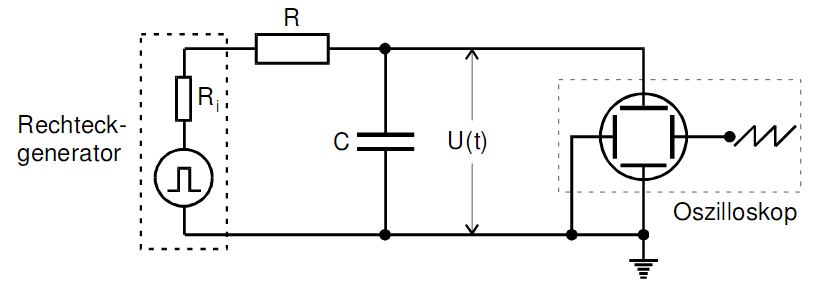
\includegraphics[scale=0.4]{aufbau.png}
  \caption{Versuchsaufbau mit Spannungsgenerator, RC-Kreis und Oszilloskop \cite{Quelle}}
  \label{aufbau}
\end{figure}
Im Versuch wird zunächst die Zeitkonstante des RC Gliedes bestimmt, wozu mit dem
Generator eine Rechteckspannung in den RC-Kreis eingespeist wird. Die Ausgangsspannung
wird anschließend am Oszilloskop in Abhängigkeit der Zeit dargestellt.
Hier ist besonders der Auf- und Entladevorgang des Kondensators von Interesse. Steigt
der auf dem Oszilloskop zu sehende Graph auf die Spannungsamplitude an, stellt dies den
Aufladevorgang des Kondensators dar. Hat dieser das Maximum erreicht, ist auf dem
Graphen eine fallende Funktion zu sehen, die sich asymptotisch der Nullinie nähert.
Dies wiederum stellt den Entladevorgang dar.
Für eine zur Auswertung geeigneten Darstellung, sollte hierbei darauf geachtet werden,
dass sich die abgelesene Spannung um den Faktor fünf bis zehn ändert. Ist dies am Oszilloskop
entsprechend eingestellt, werden zwischen dem Spannungsmaximum und Minimum 30 Messwerte
abgelesen. Anschließend wird das erhaltene Bild abgespeichert.
\\
\\
Im zweiten Teil der Durchführung wird die Frequenzabhängigkeit der Spannungsamplitude am Kondensatort
gemessen.
Hierzu wird am Generator eine Sinusspannung eingestellt und wiederum die Ausgangsspannung $U_\symup{C}(t)$
am Kondensator gemessen. Um die Auswertung möglichst genau durchführen zu können, werden Werte für $U_\symup{C}$
zwischen $\SI{10}{\Hz}$ und $\SI{30}{\kilo\Hz}$ gemessen.
\\
\\
Des Weiteren wird die frequenzabhängige Phasenverschiebung zwischen Generator- und Kondensatorspannung bestimmt.
Hierzu wird der zweite Kanal des Oszilloskops verwendet, in den die Generatorspannung $U_\symup{G}$ eingespeist wird.
Somit zeigen sich , wie in \ref{phasenverschiebung} zu sehen, zwei Spannungsverläufe im Oszilloskop,
deren Werte zur Berechnung der Phasenverschiebung abgelesen werden können.
Hierbei ist der Wert a die Breite die zwischen den beiden Nulldurchläufen der Spannungen abgelesen werden kann und
b die Schwingungsdauer der Generatorspannung. Gemessen werden hier ebenfalls wieder Werte zwischen $\SI{10}{\Hz}$ und
$\SI{30}{\kilo\Hz}$.
Die Phasenverschiebung $\phi$ kann mit folgender Formel anschließend berechnet werden:
\begin{equation*}
  \phi = \frac{a}{b}2\pi .
\end{equation*}
\begin{figure}[h!]
  \centering
  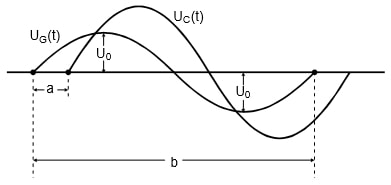
\includegraphics[scale=0.7]{phasenverschiebung.jpg}
  \caption{Darstellung der Generator- und Kondensatorspannung zur Bestimmung der Phasenverschiebung \cite{Quelle}}
  \label{phasenverschiebung}
\end{figure}
Zuletzt wird der RC-Kreis auf seine Eigenschaft als Integrator hin untersucht. Diese Untersuchung findet
qualitativ statt. Am Generator werden nachheinander Sinus-, Rechteck- und Dreieckspannung eingespeist.
Am Oszilloskop werden sowohl die Spannungsverläufe am Kondensator als auch der Spannungverlauf der Generatorspannung
abgebildet. Zu beachten ist hierbei, dass eine hinreichend große Eingangsfrequenz am Spannungsgenerator eingestellt
wird. Im Versuch wurde eine Eingangsspanung von $\SI{100}{\kilo\Hz}$ verwendet. Zur Auswertung werden die Abbildungen
der beiden Ausgangsspannungen miteinander verglichen. Die Funktion der Kondensatorspannung wird dabei das Integral
der Generatorspannung darstellen.
Alle drei Darstellungen der Spannungsverläufe werden anschließend abgespeichert.

\section{Auswertung}
\subsection{Entladevorgang eines Kondensators}

\begin{table}
  \centering
  \caption{Messwerte: Entladung eines Kondensators.}
  \label{table1}
  \begin{tabular}{c c}
    \toprule
    $t$ / ms & $U(t)$ / mV \\
    \midrule
    -5.500 & 720\\
    -5.400 & 500\\
    -5.300 & 320\\
    -5.200 & 160\\
    -5.100 & 20\\
    -5.000 & -120\\
    -4.900 & -220\\
    -4.800 & -320\\
    -4.700 & -400\\
    -4.600 & -460\\
    -4.500 & -560\\
    -4.400 & -620\\
    -4.300 & -660\\
    -4.200 & -700\\
    -4.100 & -740\\
    -4.000 & -800\\
    -3.900 & -820\\
    -3.800 & -840\\
    -3.700 & -860\\
    -3.600 & -880\\
    -3.500 & -900\\
    -3.400 & -920\\
    -3.300 & -940\\
    -3.200 & -940\\
    -3.100 & -960\\
    -3.000 & -960\\
    -2.900 & -980\\
    -2.800 & -980\\
    -2.700 & -980\\
    \bottomrule
  \end{tabular}
\end{table}

Bei der ersten Methode zur Bestimmung von $RC$ (Zeitkonstanten) wird der Entladevorgang eines Kondesators
über einen Widerstand beobachtet. Zunächst werden die Werte so im Graphen verschoben, sodass $U(t=0)=U_\symup{max}$
und $U(t \to \infty) = 0$ gilt.

\begin{figure}
  \centering
  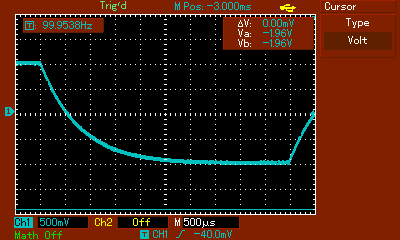
\includegraphics[scale = 0.5]{Bild1.png}
  \caption{Entladevorgang eines Kondensators.}
  \label{Bild1}
\end{figure}

\begin{figure}
  \centering
  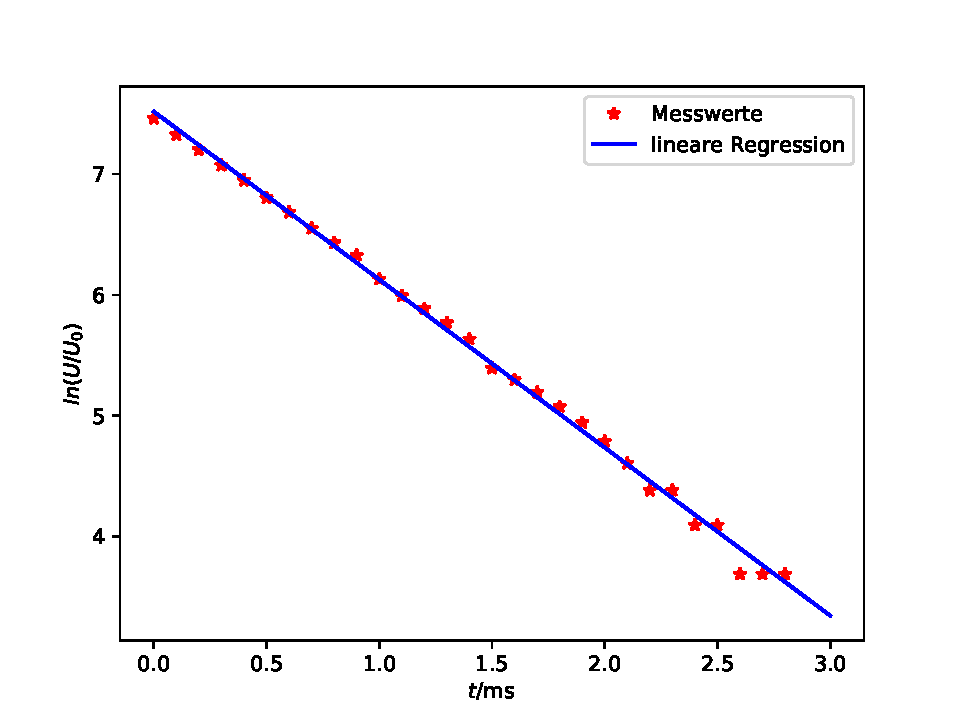
\includegraphics[scale = 0.7]{plotA.pdf}
  \caption{Messwerte und lineare Regression zur Entladung eines Kondensators.}
  \label{PlotA}
\end{figure}

Aus dem Diagramm aus Abbildung \ref{Bild1} werden 30 Wertepaare entnommen,
die Spannngen logarithmiert und in die Abbildung \ref{PlotA} eingetragen. Mit den Wertepaaren wird eine
lineare Regression durchgeführt, wobei die Steigung $m$ und der y-Achsenabschnitt $b$ wie folgt definiert sind:

\begin{align*}
  m &= - \frac{1}{RC} \\
  b &= ln(Q(0))
\end{align*}

wobei $R$ den Widerstand, $C$ die Kapazität des Kondensators, $Q(0)$ die Ladung des Kondensators zum Zeitpunkt
$t=0$ beschreibt. Mit Hilfe der linearen Regression werden die Werte für $m$ und $b$ ermittelt

\begin{align*}
  m &= \SI{-1391(14)}{\per\second} \\
  b &= \SI{0.608(23)}{} \, .
\end{align*}

Mit

\begin{equation*}
  RC = -\frac{1}{m} \, ,
\end{equation*}

folgt direkt

\begin{equation*}
  RC = \SI{0.719(7)}{\milli\second} \, ,
\end{equation*}

mit
\begin{equation*}
  \Delta RC = \frac{1}{m^2}\Delta m
\end{equation*}

\subsection{Frequenzabhängigkeit der Amplitude}

Bei der zweiten Methode zur Bestimmung der Zeitkonstanten $RC$ wird die Abhängigkeit der
Amplitude $A(\nu)$ von der Frequenz ausgenutzt. Die Messwerte werden wieder in ein Diagramm eingetragen
und es wird eine Regression der Form

\begin{equation*}
  \frac{A(\nu)}{U_0} = \frac{1}{\sqrt{1+(2 \pi \nu RC)^2}}
\end{equation*}

durchgeführt, wobei $U_0$ die Amplitude der ungedämpften Schwingung ist.
Die Regression ergibt den Wert der Zeitkonstanten

\begin{equation*}
  RC = \SI{0.771(8)}{\milli\second}.
\end{equation*}

\begin{figure}
  \centering
  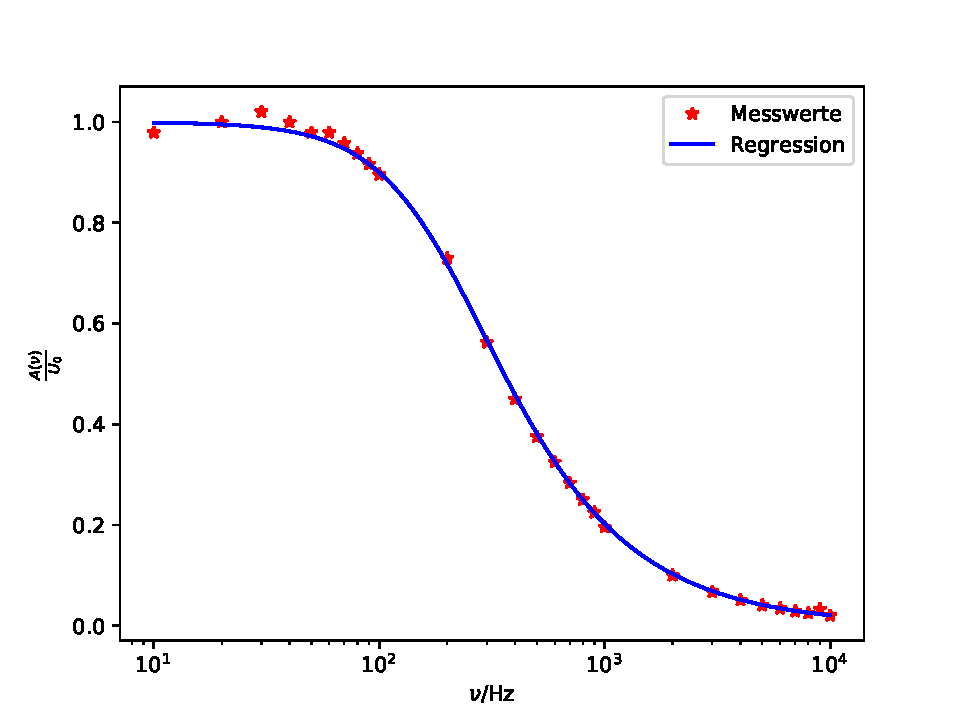
\includegraphics[scale = 0.7]{plotB.pdf}
  \caption{Amplitude $A(\nu)$ in Amhängigkeit der Frequenz $\nu$}
  \label{Plot2}
\end{figure}

\begin{table}
  \centering
  \caption{Messwerte: Frequenzabhängigkeit der Amplitude.}
  \label{table2}
  \begin{tabular}{c c}
    \toprule
    $\nu$ /Hz & $U$ /mV \\
    \midrule
    10 & 940\\
    20 & 960\\
    30 & 980\\
    40 & 960\\
    50 & 940\\
    60 & 940\\
    70 & 920\\
    80 & 900\\
    90 & 880\\
    100 & 860\\
    200 & 700\\
    300 & 540\\
    400 & 432\\
    500 & 360\\
    600 & 312\\
    700 & 272\\
    800 & 240\\
    900 & 216\\
    1000 & 188 \\
    2000 & 96\\
    3000 & 64.4\\
    4000 & 48.8\\
    5000 & 39.2\\
    6000 & 32.8\\
    7000 & 27.6\\
    8000 & 24.0\\
    9000 & 31.6\\
    10000 &  19.2\\
    \bottomrule
  \end{tabular}
\end{table}

\subsection{Frequenzabhängikeit der Phasenverschiebung}


Zunächst in wird der Phasenunterschied $\Delta\phi$ mit Hilfe der Formel

\begin{equation*}
  \Delta\phi = \frac{\Delta t}{T} \cdot 2 \pi
\end{equation*}

berechnet. Analog zu den Methoden vorher, werden die Werte in ein Diagramm eingetragen und eine
Regression der Form

\begin{equation*}
  \Delta\phi(\nu) = \arctan (-2 \pi \nu RC)
\end{equation*}

durchgeführt. Die Regression liefert den Wert für dei Zeitkonstante

\begin{equation*}
  RC = \SI{0.767(25)}{\milli\second}
\end{equation*}

\begin{figure}
  \centering
  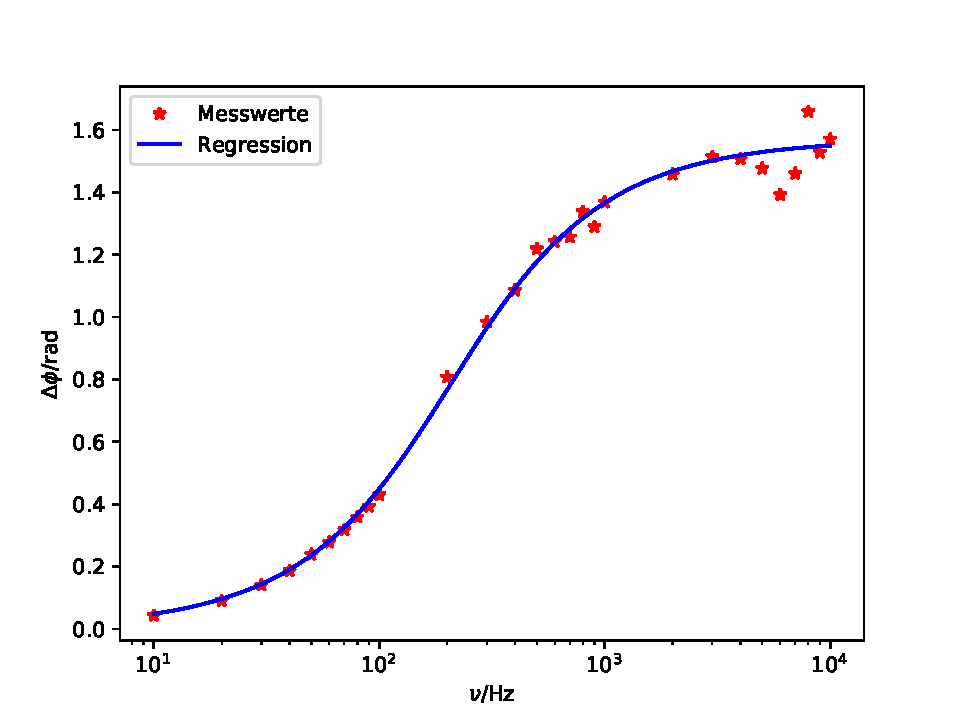
\includegraphics[scale = 0.7]{plotC.pdf}
  \caption{Phasenverschiebung $\Delta\phi (\nu)$ in Abhängigkeit der Frequenz $\nu$ }
  \label{Plot3}
\end{figure}

\begin{figure}
  \centering
  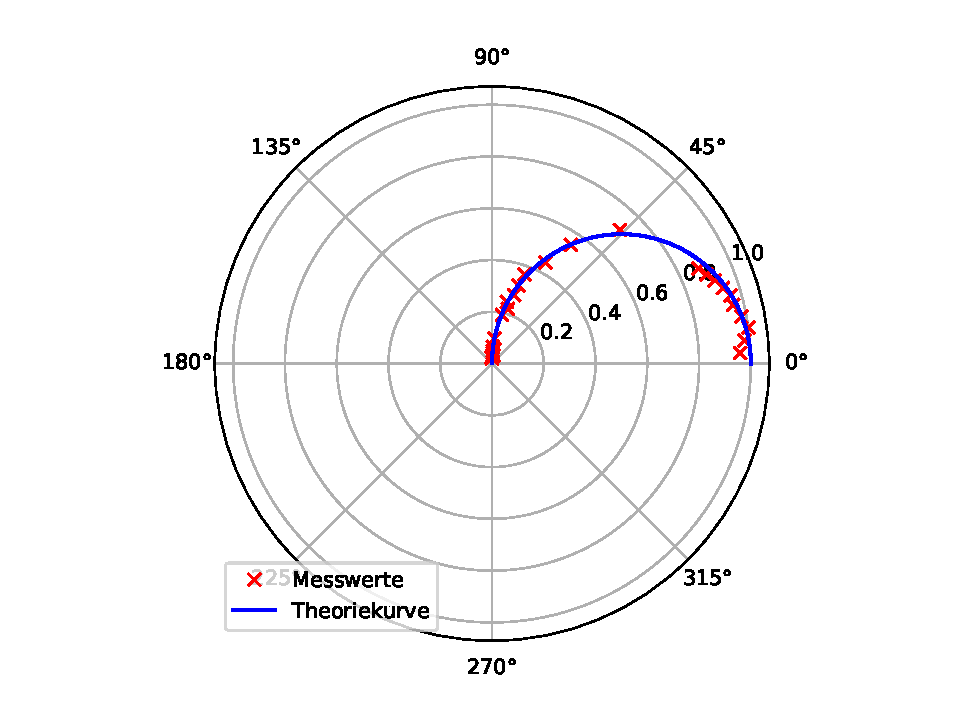
\includegraphics[scale = 0.7]{polar2.pdf}
  \caption{Phasenverschiebung $\Delta\phi $ in Abhängigkeit von $\frac{U_c}{U_0} $}
  \label{polar}
\end{figure}

\begin{table}
  \centering
  \caption{Messwerte: Frequenzabhängigkeit der Phasenverschiebung. Wobei $\Delta t$ die Zeitdifferenz
  zwischen der gedämpften und ungedämpften Schwingung und $T$ die Periodendauer einer Schwingung ist.}
  \label{table3}
  \begin{tabular}{c c c}
    \toprule
    $\nu$ / Hz & $\Delta t$ / $\mu$ s & $T$ / ms \\
    \midrule
    10 & 680 & 100\\
    20 & 720 & 50\\
    30 & 740 & 33\\
    40 & 740 & 25\\
    50 & 760 & 20\\
    60 & 740 & 16.72\\
    70 & 724 & 14.32\\
    80 & 708 & 12.4\\
    90 & 700 & 11.2\\
    100 & 684 & 10\\
    200 & 640 & 4.98\\
    300 & 520 & 3.32\\
    400 & 432 & 2.5\\
    500 & 384 & 1.98\\
    600 & 328 & 1.66\\
    700 & 288 & 1.44\\
    800 & 264 & 1.24\\
    900 & 232 & 1.13\\
    1000 & 216 & 0.992\\
    2000 & 116 & 0.500\\
    3000 & 80 & 0.332\\
    4000 & 60 & 0.250\\
    5000 & 47 & 0.200\\
    6000 & 37 & 0.167\\
    7000 & 33 & 0.142\\
    8000 & 33 & 0.125\\
    9000 & 27 & 0.111\\
    10000 & 25 & 0.100\\
    \bottomrule
  \end{tabular}
\end{table}

\newpage

\subsection{RC-Kreis als Integrator}

Man kann für bestimmte Bedingungen den RC-Kreis auch als Integrator dienen. Eine Bedingung dafür
ist eine hohe Frequenz, in unserem Versuch werden die Bilder mit einer Frequenz von 100 kHz
aufgenommen. Folgend beschreiben die gelben Funktionen die Ausgangsspannung und die blauen Funktionen
die Spannung über den RC-Kreis.

\begin{figure}[h!]
  \centering
  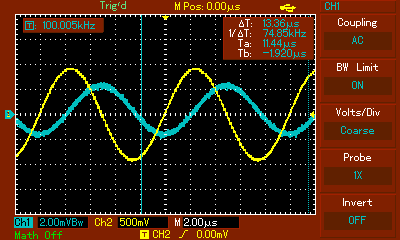
\includegraphics[scale = 0.6]{Bild2.png}
  \caption{RC-Kreis als Integrator, Sinusschwingung.}
  \label{Integrator1}
\end{figure}

\begin{figure}[h!]
  \centering
  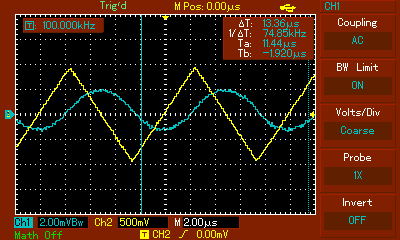
\includegraphics[scale = 0.6]{Bild4.png}
  \caption{RC-Kreis als Integrator, Dreiecksspannung}
  \label{Integrator2}
\end{figure}

\begin{figure}[h!]
  \centering
  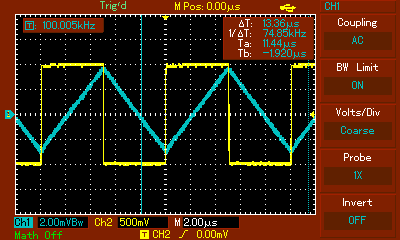
\includegraphics[scale = 0.6]{Bild5.png}
  \caption{RC-Kreis als Integrator, Rechteckschwingung}
  \label{Integrator3}
\end{figure}

In Abbildung \ref{Integrator1} wird eine Sinusspannung durch den Spannungsgenerator erzeugt.
Es lässt sich erkennen, dass die blaue Spannung eine  negative Cosinusfunktion (an der x- Achse gespiegelt) darstellt,
welchemathematisch auch das Integral einer Sinusfunktion ist.

In Abbildung \ref{Integrator2} wird eine Dreiecksspannung erzeugt. Hier lässt sich erkennen, dass die
Integrationsfunktion aus Parabeln besteht. Mathematisch gesehen wird aus einer Geraden nach der Integration
eine Parabel, welches den RC-Kreis aus Integrator bestätigt.

In Abbildung \ref{Integrator3} wird eine Rechteckschwingung angelegt. Mathematisch gesehen, ist
das Integral einer konstanten Funktion eine Gerade, wobei der Wert der Funktion der Steigung entspricht.
Hier ist zu erkennen, dass aus einer Rechteckfunktion nach der Integration eine Dreiecksfunktion wird,
welche aus unendlich vielen Geraden besteht. Auch hier lässt sich die FUnktion des RC-Kreises als
Integrator gut erkennen.

\section{Diskussion}

\begin{table}
  \centering
  \caption{Vergleich der Werte für die Zeitkonstante}
  \label{Vergleich}
  \begin{tabular}{c c c c}
    \toprule
    & Entladung & Amplitude & Phase \\
    \midrule
    $RC$ / ms & \num{0.719(7)} & \num{0.771(8)} & \num{0.767(25)} \\
    \bottomrule
    \end{tabular}
\end{table}

In Tabelle \ref{Vergleich} sind die einzelnen experimentell ermittelten Zeitkonstanten aufgelistet.
Zu erkennen ist, dass alle Zeitkonstanten in der Gleichen Größenordnung liegen. Dennoch gibt es
Abweichung, wobei dort auch systematische Fehler vorhanden sind, denn bei allen Versuchen wird der
Innenwiderstand des Generators vernachlässigt.
Weitere Fehler lassen sich auf Messfehler zurückführen. Diese haben ihren Ursprung beim Errechnen der Werte
des Oszilloskops, da bei größerern Frequenzen die zu messenden Größen immer kleiner werden und das
Oszilloskop beispielsweise bei der Messung der Amplituden nur in 20mV-Schritten messen kann.
\newpage
\nocite{}
